Para determinar la carga especifica del electrón, se emplea un haz de
electrones que se desplaza con una velocidad \(v\) perpendicular a un campo
magnético generado por un par de Bobinas de Helmholtz.
Estas bobinas representan la configuración más simple capaz de generar un campo
magnético prácticamente uniforme y constante.
La configuración consiste en dos bobinas circulares coaxiales de igual radio,
con una separación entre sus planos igual al radio de las mismas.

\begin{figure}[htbp!]
  \centering
  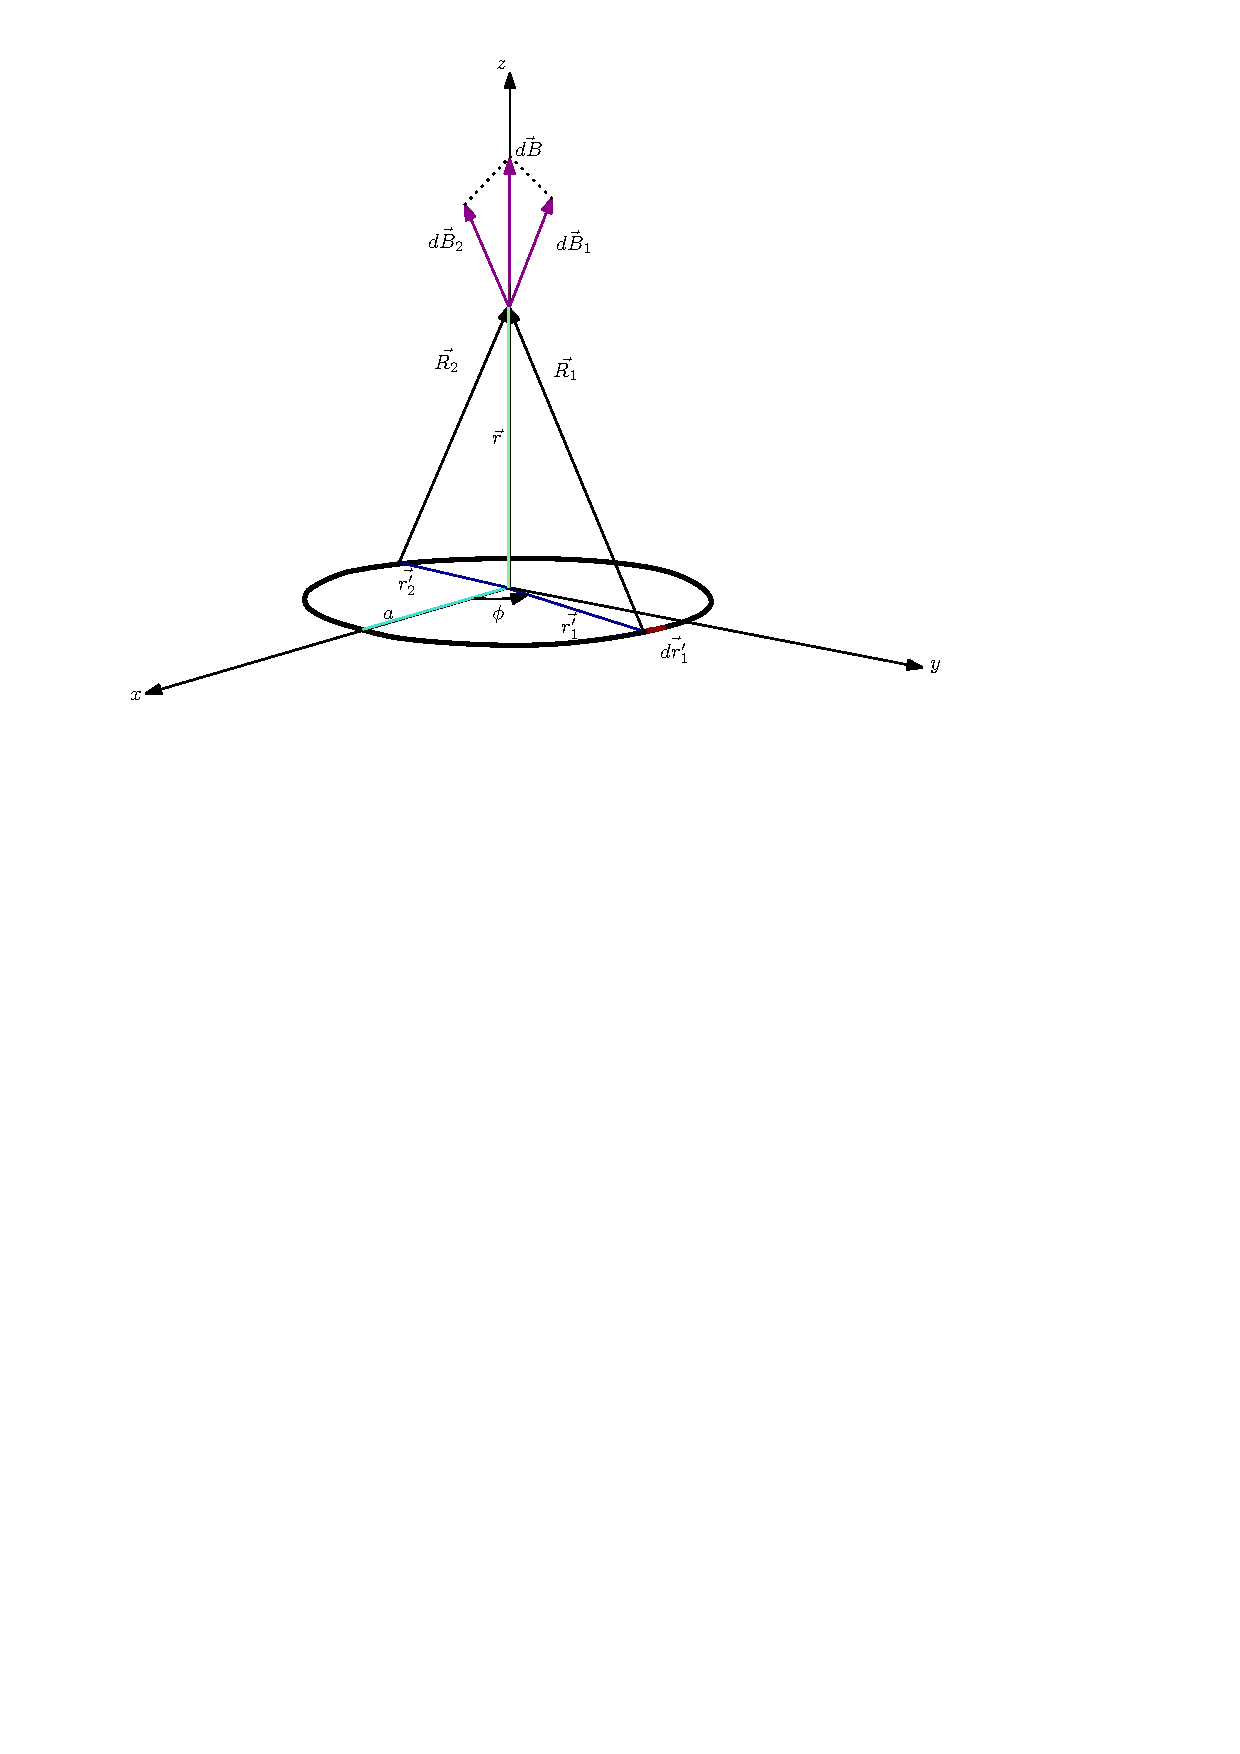
\includegraphics[width=0.8\linewidth]{./images/loop-field.pdf}
  \caption{Campo magnético de una espira.}
  \label{fig:loop}
\end{figure}

Para calcular el campo magnético generado por estas bobinas, primero se
determina el campo producido por una de ellas.
En este caso, se considera una espira por la que circula una corriente eléctrica
constante \(I\) en el tiempo.
Partimos de la expresión diferencial de la ley de Biot-Savart \cite{jackson-1998}:

\begin{equation}\label{eq:Biot-Savart}
  d\mathbf{B}(\mathbf{r}) = \frac{\mu_0 I}{4 \pi} \frac{d\mathbf{l} \times \mathbf{R}}{R^{3}}
\end{equation}

Donde:
\begin{itemize}
  \item $d\mathbf{l}=a d\phi \hat{\phi}$
  \item $\mathbf{R}=\mathbf{r}-\mathbf{r'}$
  \item $\mathbf{r}=z\hat{e_{z}}-a\hat{e_{\rho}}$
  \item $R=\sqrt{z^{2}+a^{2}}$
\end{itemize}

Por lo que reemplazando se tiene que:
\begin{equation}
  d\mathbf{B}(\mathbf{r}) = \frac{\mu_{0}I}{4\pi} \frac{(a d\phi z \hat{\rho}) + (a^{2}d\phi \hat{z})}{(z^{2}+a^{2})^{3/2}}
\end{equation}

Al integrar se obtiene el valor de $\mathbf{B}(\mathbf{r})$ y por la simetría
del problema se evidencia que $\mathbf{B}(\mathbf{r}) = B(r)\hat{z}$,
por lo que se obtiene:
\begin{equation}
  \mathbf{B}(\mathbf{r}) = \frac{\mu_{0}I}{4 \pi} \frac{a^{2}}{(z^{2}+a^{2})^{3/2}} \hat{e_{z}} \int _{0}^{2 \pi} d\phi
\end{equation}

Lo que da como resultado:
\begin{equation}
  \mathbf{B}(\mathbf{r}) = \frac{\mu_{0}I}{2} \frac{a^{2}}{(z^{2}+a^{2})^{3/2}} \hat{e}_{z}
  \label{eq:Campo_magnetico_espira}
\end{equation}

\begin{figure}[htbp!]
  \centering
  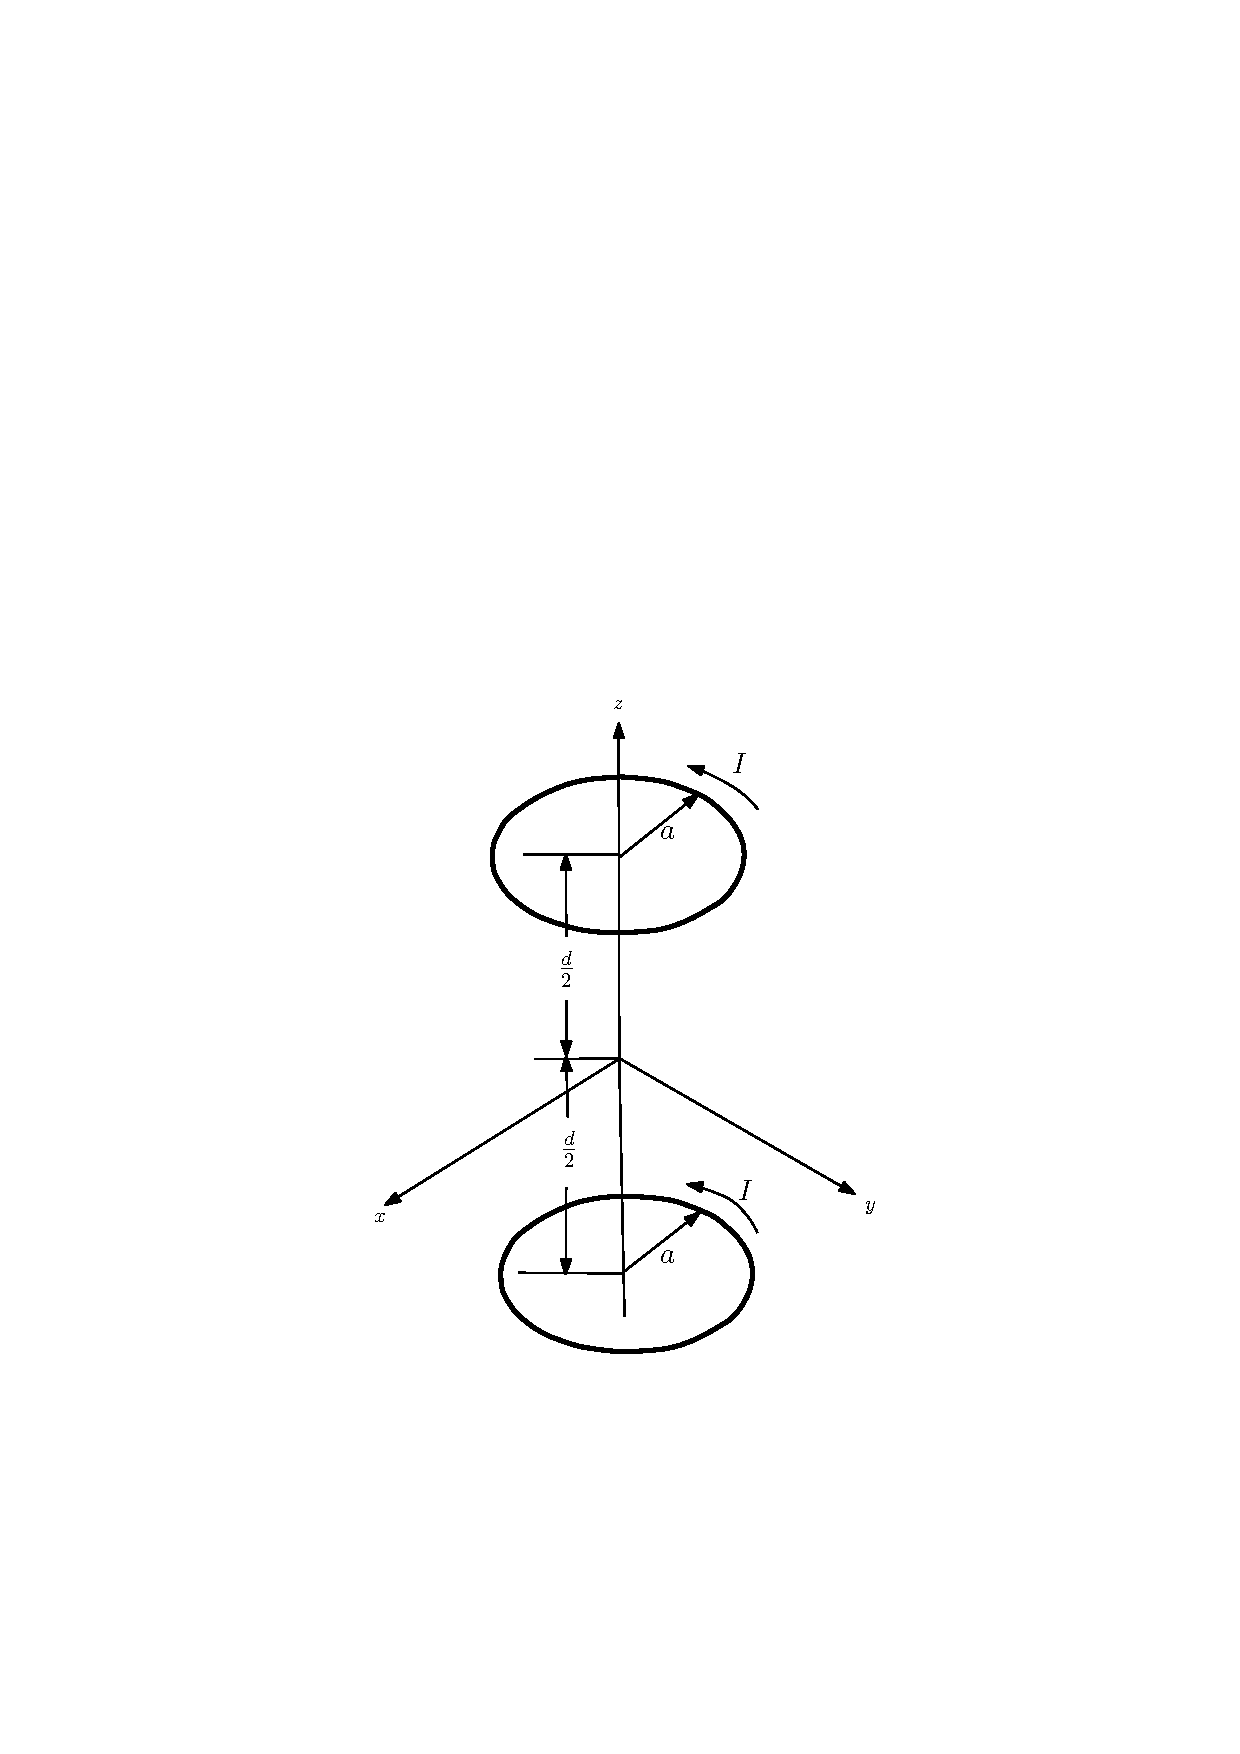
\includegraphics[width=0.6\linewidth]{./images/two-loops.pdf}
  \caption{Corriente en dos espiras.}
  \label{fig:two-loops}
\end{figure}

\begin{figure}[htbp!]
  \centering
  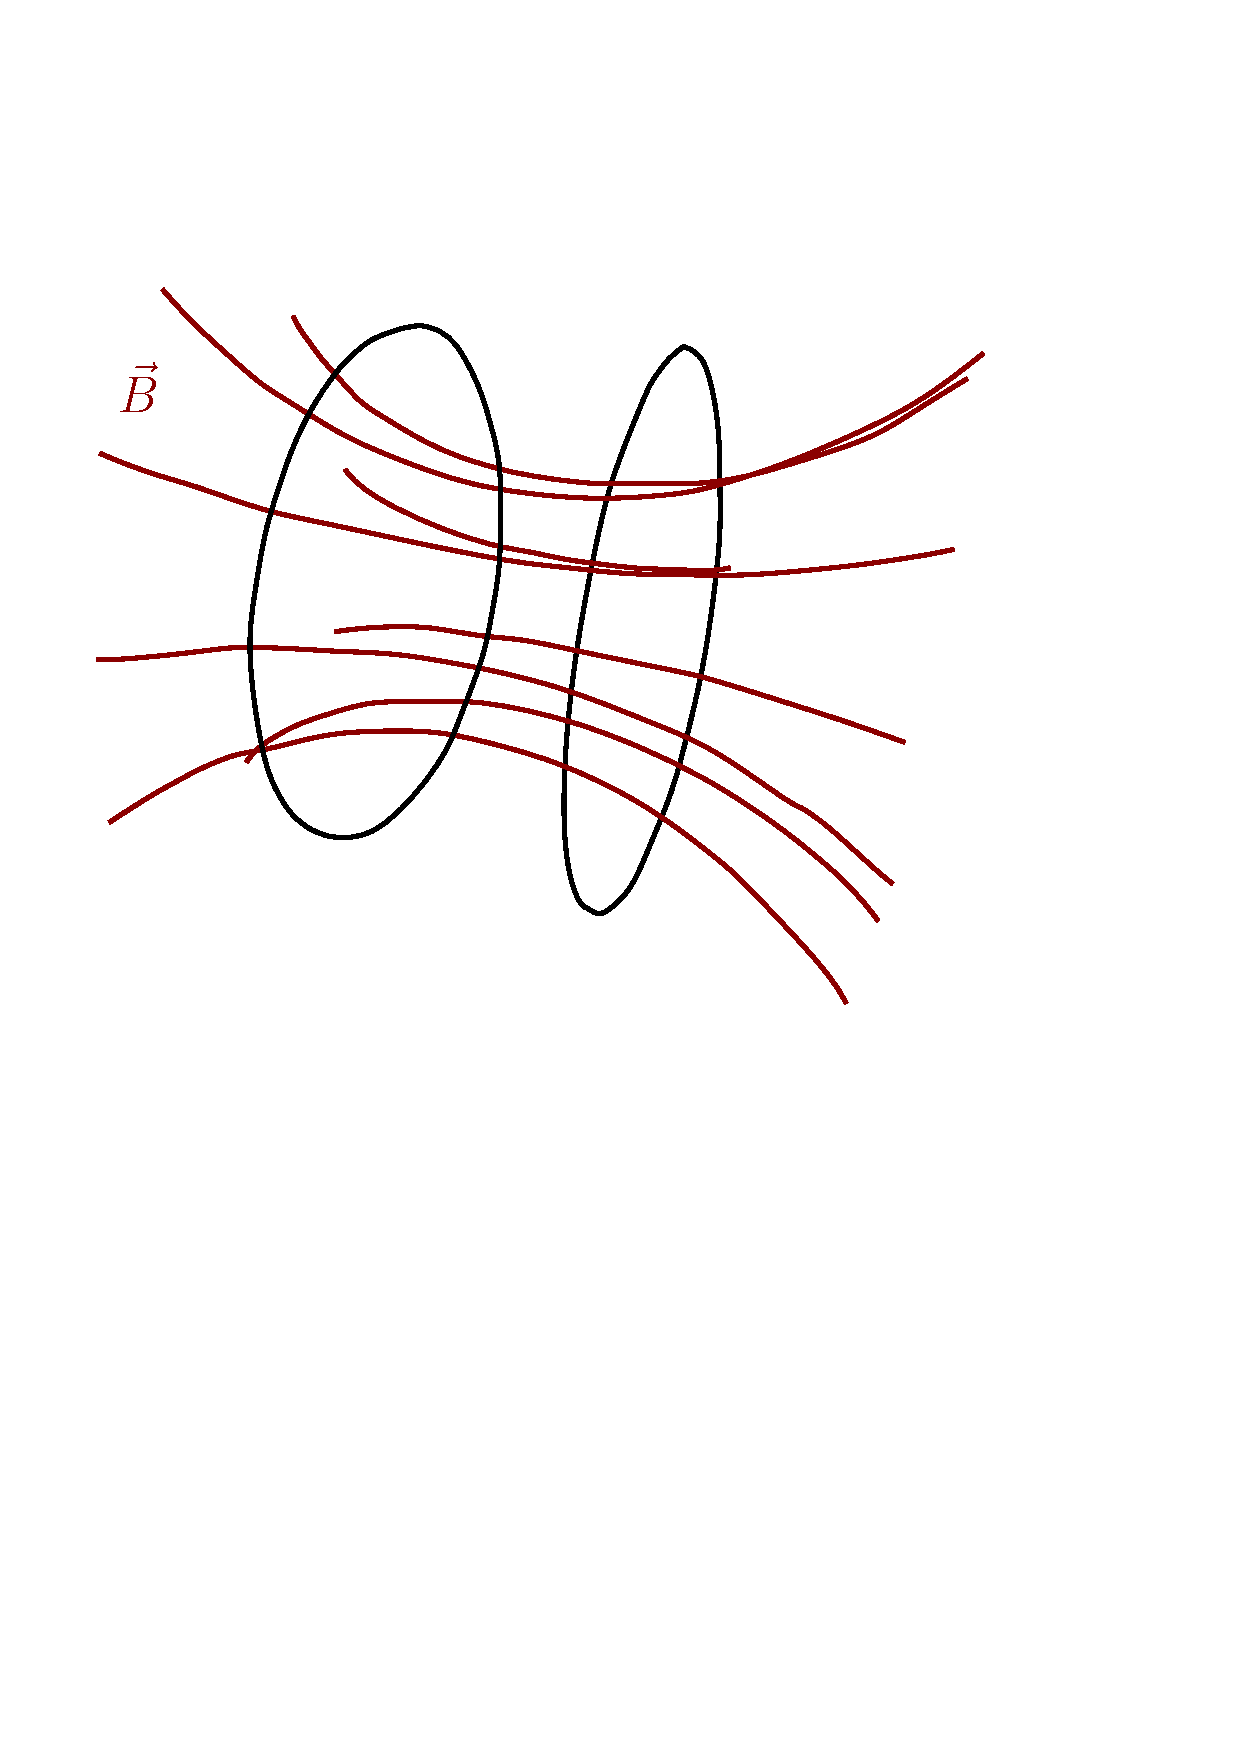
\includegraphics[width=0.6\linewidth]{./images/coils-field.pdf}
  \caption{Campo magnético entre dos espiras circulares.}
  \label{fig:coils-field}
\end{figure}

El campo magnético $\mathbf{B}$ producido por dos espiras, como se observa en la
\cref{fig:two-loops}, donde circula una corriente estática $I$ en cada una de
las espiras, se calcula sumando dos componentes del vector $\mathbf{B}$ de
acuerdo al resultado de la \cref{eq:Campo_magnetico_espira}.
Como resultado, se obtendrán dos términos iguales, considerando que las espiras
se encuentran localizadas en \(z = -d/2\) y \(z = d/2\).

\begin{equation}
  \begin{aligned}
    \mathbf{B}_{z}(\rho=0,z) &= \frac{\mu_{0} I a^{2}}{2} \left[ \frac{1}{\left((z-\frac{d}{2})^{2} + a^{2}\right)^{3/2}} \right.\\
                             &\quad \left.+ \frac{1}{\left((z+\frac{d}{2})^{2} + a^{2}\right)^{3/2}} \right] \hat{e}_{z}
                             \label{Campo_magnetico_2espiras}
  \end{aligned}
\end{equation}

Para el caso del montaje experimental, las bobinas tienen una separación igual a
su radio, por lo que \( d = a \).
Además, el haz de electrones se ubica en el centro de las bobinas, es decir,
\( z = 0 \). Teniendo en cuenta todas estas consideraciones, se llega a que el
campo magnético producido por las bobinas en el haz de electrones es:

\begin{equation}
  \mathbf{B}_{z}(\rho=0, z=0) = \frac{8 n \mu_{0} I}{5 \sqrt{5} R}
  \label{eq:Campo_magnetico_enHaz}
\end{equation}

\begin{equation}
  \mathbf{B}(\mathbf{r}) = \frac{\mu_{0}I}{2} \frac{a^{2}}{(z^{2}+a^{2})^{3/2}} \hat{e}_{z}
\end{equation}

donde \( R = a \).

\begin{figure}[htbp!]
  \centering
  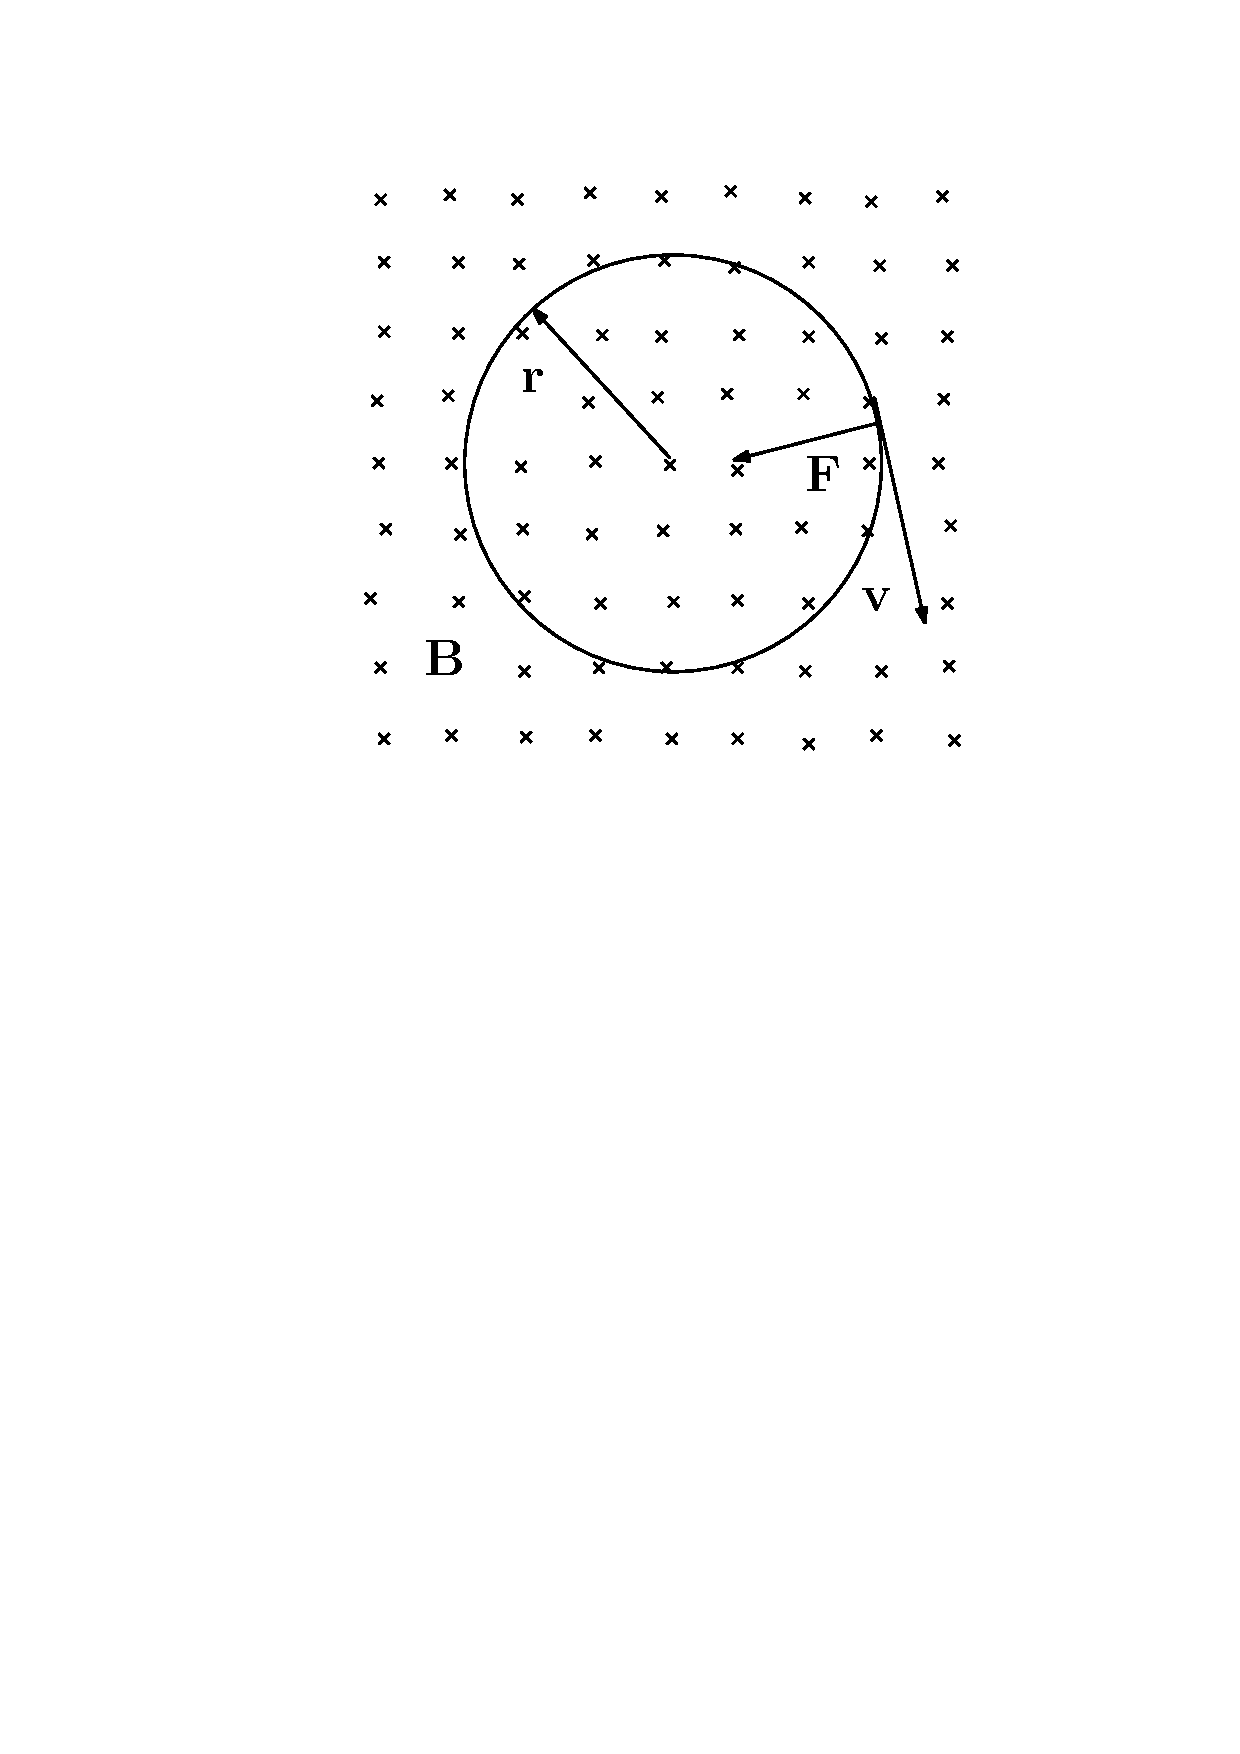
\includegraphics[width=0.8\linewidth]{./images/electron-path.pdf}
  \caption{Trayectoria del haz de electrones}
  \label{fig:haz_elelctrones}
\end{figure}

Dado que el electrón, con carga \( e \), se mueve perpendicularmente al campo
magnético, está sujeto a la fuerza de Lorentz, cuya magnitud está dada por:

\begin{equation}
  F = e v B
  \label{eq:FuerzaLorentz}
\end{equation}

Debido a que la fuerza de Lorentz es perpendicular a la velocidad y al campo
magnético, genera un movimiento circular en el haz de electrones, por lo que
también actúa como una fuerza centrípeta:

\begin{equation}
  F = m_{e} \frac{v^{2}}{r}
  \label{eq:Fuerzacentripeta}
\end{equation}

Igualando las \cref{eq:FuerzaLorentz,eq:Fuerzacentripeta}, se obtiene una
relación carga-masa en función de la velocidad, el campo magnético y el radio
del haz de electrones:

\begin{equation}
  \frac{e}{m_{e}} = \frac{v}{r B}
  \label{eq:Primera_carga-masa}
\end{equation}

Sin embargo, la velocidad con la que viaja el haz de electrones es desconocida.
Para determinarla, se recurre a la conservación de la energía.
En el experimento, los electrones son acelerados en un tubo de rayo electrónico
filiforme por una diferencia de potencial \( U \), de modo que la energía
eléctrica se transforma en energía cinética:

\begin{equation}
  \begin{aligned}
    e U &= \frac{1}{2} m_{e} v^{2} \\
    \Rightarrow \frac{e}{m_{e}} &= \frac{v^{2}}{2 U}
  \end{aligned}
  \label{eq:Segunda_carga-masa}
\end{equation}

Igualando las ecuaciones \cref{eq:Primera_carga-masa,eq:Segunda_carga-masa},
se obtiene que la velocidad es \( v = \frac{2 U}{r B} \), y finalmente,
se llega a que la carga específica del electrón es:

\begin{equation}
  \frac{e}{m_{e}} = \frac{2 U}{(r B)^{2}}
  \label{eq:carga-masa}
\end{equation}
